% !Mode:: "TeX:UTF-8"
\chapter{视频编码原理与关键技术}
\label{cha:c2}
在正文之前,首先申明以下用词:1) 统一使用视频“编码”而非视频“压缩”。在视频编解码领域,“编码”与“压缩”表达相同的含义,都指经过预测、变换量化、熵编码等操作达到减小数据冗余、压缩视频数据量的目的。编码是手段,压缩是目的,按照习惯统一使用视频编码这一表述,类似地,使用编码标准、编码方案、编码效率等表述;2) 为了直接体现出编码标准的发展历程,不使用高级视频编码(Advanced Video Coding,AVC)、高性能视频编码(High Efficiency Video Coding,HEVC)和多功能视频编码(Versatile Video Coding,VVC)的表述,统一使用 H.264、H.265 和 H.266,两类表述在含义上并无差异;3) 由联合专家组维护的各标准参考模型随着版本迭代可能存在不同的命名,例如 H.266 的参考模型在早期曾称为 JEM(Joint Exploration Model),本文中统一使用以下命名:用于 H.264 的 JM(Joint Test Model)模型、用于 H.265 的 HM(HEVC Test Model)模型以及用于 H.266 的 VTM(VVC Test Model)模型。

\section{视频编码技术发展历史}

\section{预测编码技术}
预测编码是 H.26X 系列编码标准中的重要组成部分之一。视频信号表现出很强的空间相关性和时间相关性,即在空间上相邻像素点之间的亮度或色差值相近,在时间上同一区域相邻两帧之间的像素点亮度或色差值相近。使用帧内和帧间预测技术可以准确地对待编码数据进行预测,进而编码预测值与原始像素值的残差,极大地减少视频信号的时空冗余。预测编码的基本流程如图 \ref{fig:PredicitonOverview} 所示。对于待预测像素 $x(n)$,首先利用已重建的像素结合特定的预测模式得到预测值 $p(n)$,然后计算预测残差 $e(n)$,最后对 $e(n)$ 进行变换、量化、熵编码,同时使用去量化、逆变换后的重建值 $e^{'}(n)$ 与预测值 $p(n)$
\begin{figure}[htb]
    \centering
    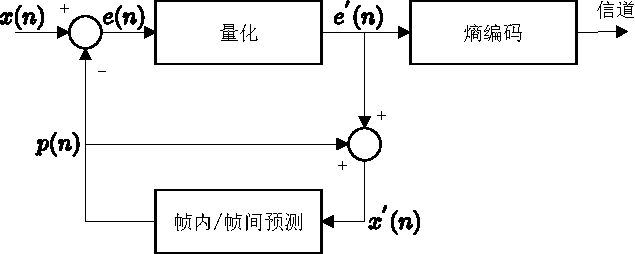
\includegraphics{PredicitonOverview.pdf}
    \caption{H.26X 预测编码的基本流程}
    \label{fig:PredicitonOverview}
\end{figure}
\subsection{帧内预测}
\subsection{帧间预测}

\section{变换与量化技术}
\subsection{变换编码}
\subsection{量化}

\section{环路后处理技术}
\subsection{去方块滤波}
\subsection{样点自适应补偿}

\section{熵编码技术}
\subsection{变长编码在视频编码中的应用}
\subsection{算术编码在视频编码中的应用}
\subsection{模式依赖的编码顺序}

\section{率-失真优化技术}
不论是视频编码标准还是各类网络传输协议标准,标准中制定的往往只是各类语法和语义(部分包含同步规则和检错纠错规则),只要是符合标准语法语义的码流都能称为符合某视频编码标准。例如在使用 H.265 进行编码时,若将最小预测单元限定为 32x32(HM 默认配置是 4x4),编码效率与失真度可以预见甚至不如简单的 M-JPEG(Motion Joint Photographic Experts Group)。因此,如何在标准的编码框架下得到最优的编码效率与失真度的平衡是编码算法研究的核心内容之一,寻找折衷点的过程被称为率-失真优化(Rate-Distortion Optimization,RDO)。
% 有各种级别的率-失真优化,片层级,CTU 级,PU 级
% 不同的软件有不同的方案,介绍 HM
% 标准只规定了码流语义 编码可以自由发挥 就算我全用64x64质量超低也能叫HEVC 所以需要优秀的压缩率-失真的折衷策略
% 也是业界在竭力优化的核心内容

\section{软、硬件视频编码开源项目}
互联网开源精神是当今学术界与工业界发展的重要推手,而视频编解码这一涉及到成像系统、生物信息、数学、统计学、计算机以及集成电路的庞大学科,如果没有一个系统的开源项目让各学科的研究人员参与进来,而是由单一的某一组织闭门造车是无法得到长足发展的。本小节总结了目前常用的软、硬件视频编码开源项目,本课题就是基于其中部分项目开展的。
\subsection{软件视频编码开源项目}
\begin{itemize}
    \item JM

    JM 是制定 H.264 标准的联合开发组(Joint Video Team,JVT)负责维护的 H.264 编解码参考软件\upcite{AVCsoftwareJM}。JM 是学术界常用的编码器,其实现了 H.264 的所有特性,内部没有使用多线程或进行汇编层级的优化,因此其编解码速度较慢无法实现实时编码,多用于研究和测试标准性能。

    \item x264

    x264 是由 VideoLAN 维护的 H.264 编码器。x264 是工业界最常用的 H.264 编码器,其内部集成了丰富的快速、并行算法,使得编解码效率得到了极大提升,被应用在各类开源音视频处理框架中。目前最完善的多媒体处理软件 FFmpeg 在 H.264 部分就内嵌了 x264 用于编码。

    \item HM

    HM 是制定 H.265 标准的视频编码联合工作组(Joint Collaborative Team on Video Coding,JCT-VC)负责维护的 H.265 编解码参考软件\upcite{HEVCsoftwareHM16}。HM 是学术界在研究 H.265 和下一代视频编码标准时常用的编码器,其实现了 H.265 的所有特性(包括部分未写入标准的会议提案),内部没有使用多线程或进行汇编层级的优化,因此其编解码速度较慢无法实现实时编码,多用于研究和测试标准性能。

    \item VTM

    VTM 是制定 H.266 标准的联合视频探索小组(Joint Video Exploration Team,JVET)负责维护的 H.266 编解码参考软件\upcite{VVCsoftwareVTM},随着 H.266 编码提案的征集仍在快速迭代中,在 H.266 标准探索的初期曾称为 JEM。VTM 是联合小组在制定下一代视频编码标准 H.266 时使用的编码器,用于测试编码提案的性能。
\end{itemize}

\subsection{硬件视频编码开源项目}
\begin{itemize}
    \item OpenASIC Encoder RTL IP

    OpenASIC H.264/H.265 Encoder RTL IP 是由复旦大学微电子学院视频图像处理科研团队发布的 H.264/H.265 开源 RTL IP,由开源芯片社区 OpenASIC 共同维护。其中 H.264 Encoder RTL IP 实现了 H.264 标准编码流程,最大支持 1920x1088@30fps 实时编码,已被部分公司、研究所研究使用;H.265 Encoder RTL IP 发布了 2 个版本,实现了帧内/帧间预测、熵编码、环路后处理以及基础的码率控制,满足 400MHz 无时序违例综合,最大支持 4K@30fps 实时编码。
\end{itemize}